\documentclass[12pt]{article} 
\usepackage[margin=1in]{geometry} 
\usepackage{graphicx} 
\usepackage{hyperref} 
\usepackage{tocloft}
\usepackage{enumitem}
\usepackage{mathptmx} % Times New Roman
\usepackage{setspace}
\usepackage{fancyhdr} % Header and footer
\usepackage[indonesian]{babel}
\usepackage{caption}
\captionsetup[table]{name=Tabel}
\captionsetup[figure]{name=Gambar}

\renewcommand{\contentsname}{Daftar Isi}

\title{Laporan Evaluasi Tengah Semester\\Pemrograman Jaringan C} 
\author{Muhammad Daffa' Ashdaqfillah (5025211015)} 
\date{\today} 

\pagestyle{fancy}
\fancyhf{} % Clear existing header/footer
\rhead{Evaluasi Tengah Semester - Progjar C}
\rfoot{\thepage}
\lfoot{Muhammad Daffa Ashdaqfillah - 5025211015}
\renewcommand{\footrulewidth}{0.4pt}

\begin{document}

% Halaman Cover
\begin{titlepage}
    \centering
    {\scshape\Large Laporan Pengerjaan\par}
    \vspace{0.4cm}
    {\huge\bfseries Evaluasi Tengah Semester\par}
    \vspace{0.1cm}
    {\large\bfseries Pemrograman Jaringan C\par}
    \vspace{1cm}
    \vspace{1.5cm}
    
\includegraphics[width=0.6\textwidth]{img/logo_its.png}\par\vspace{1cm}
    \vspace{1cm}
    \vspace{1.5cm}
    {\large\bfseries Muhammad Daffa' Ashdaqfillah (5025211015)\par}
    {\scshape\LARGE Institut Teknologi Sepuluh Nopember \par}
    \vfill
    {\large Surabaya\par}
    {\large 28 Mei 2024\par}
    \end{titlepage}
\newpage

\setcounter{page}{2} % Mulai penomoran halaman setelah sampul

% Daftar Isi
\tableofcontents
\newpage

\section{Pendahuluan}

Laporan ini mengevaluasi kinerja berbagai implementasi server web, yaitu menggunakan \textit{multithreading}, \textit{multiprocessing}, dan varian \textit{secure} dari keduanya. Kode server yang dievaluasi (disajikan sebelumnya) merupakan modifikasi dari contoh yang disediakan dalam \textit{progjar5}. Server ini dirancang untuk menangani permintaan HTTP sederhana, menjadikannya dasar yang ideal untuk memahami bagaimana model konkurensi (\textit{multithreading} dan \textit{multiprocessing}) memengaruhi kinerja server dalam skenario beban kerja yang berbeda.

\subsection{Tujuan}

Tujuan utama dari evaluasi ini adalah:

\begin{enumerate}
    \item \textbf{Membandingkan Kinerja:} Menganalisis secara kuantitatif perbedaan kinerja antara model \textit{multithreading} dan \textit{multiprocessing}, baik dalam versi standar maupun yang telah diamankan (\textit{secure}).
    \item \textbf{Mengukur Skalabilitas:} Menilai bagaimana setiap implementasi server menangani peningkatan jumlah permintaan bersamaan (\textit{concurrency}).
    \item \textbf{Memahami Faktor-Faktor Kinerja:} Mengidentifikasi metrik kinerja utama yang dipengaruhi oleh pilihan model konkurensi dan keamanan, termasuk waktu respons, \textit{throughput}, dan penggunaan sumber daya.
    \item \textbf{Memberikan Rekomendasi:} Berdasarkan hasil evaluasi, memberikan rekomendasi tentang model konkurensi yang paling sesuai untuk berbagai skenario penggunaan server web.
\end{enumerate}

Evaluasi ini menggunakan Apache Benchmark (`ab`) untuk menghasilkan beban kerja yang realistis dan mengumpulkan metrik kinerja yang relevan. Laporan ini akan menyajikan hasil pengujian secara rinci, menganalisis temuan, dan memberikan kesimpulan yang bermanfaat bagi pengembangan server web yang efisien dan skalabel.
\newpage

\section{Metodologi}
\subsection{Pengaturan Eksperimen}
Uji coba dilakukan pada mesin virtual dengan spesifikasi berikut:

\begin{table}[h]
\centering
\caption{Spesifikasi Mesin Virtual}
\label{tab:vm_specs}
\begin{tabular}{|l|l|}
\hline
\textbf{Komponen} & \textbf{Spesifikasi} \\ \hline
Sistem Operasi & Linux (5.15.146.1-microsoft-standard-WSL2) \\ 
Prosesor & AMD Ryzen 7 4800H with Radeon Graphics (16 cores, 32 threads) \\
RAM & 5.5 GiB \\
Penyimpanan & 1007 GB (overlay), 340 GB (E:) \\
\hline
\end{tabular}
\end{table}

Server web dijalankan pada mesin virtual ini. Pengujian kinerja dilakukan dari mesin lain yang terhubung ke jaringan lokal yang sama. 

\begin{figure}[h!]
\centering
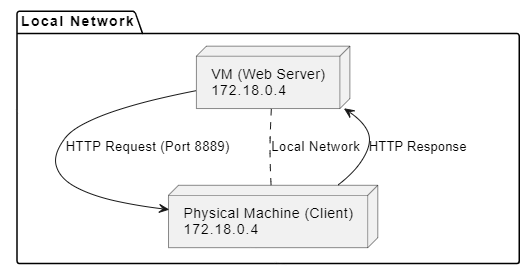
\includegraphics[width=0.8\textwidth]{img/architecture_diagram.png}
\caption{Diagram Arsitektur Eksperimen}
\label{fig:arch}
\end{figure}

Gambar \ref{fig:arch} mengilustrasikan arsitektur percobaan. Mesin penguji (client) dan mesin yang menjalankan server web (virtual machine) terhubung ke jaringan lokal yang sama. Pengujian kinerja dilakukan dengan mengirimkan permintaan HTTP ke server web menggunakan Apache Benchmark (`ab`). 

\subsection{Pengukuran Kinerja}

Pengukuran kinerja dilakukan menggunakan \textit{Apache Benchmark} (`ab`), sebuah alat yang dirancang untuk menguji kinerja server HTTP. Alat ini menghasilkan beban kerja dengan mengirimkan sejumlah permintaan HTTP ke server dan mengukur berbagai metrik kinerja. 

\subsubsection{Parameter Pengujian}

Pengujian dilakukan dengan mengirimkan 1000 permintaan (`-n 1000`) pada setiap iterasi. Tingkat konkurensi (jumlah permintaan yang dikirim secara bersamaan) divariasikan untuk melihat bagaimana kinerja server berubah seiring dengan meningkatnya beban. Tingkat konkurensi yang digunakan adalah 10, 50, 100, 150, dan 200 (`-c 10`, `-c 50`, dst.).

\subsubsection{Perintah yang Digunakan}

Perintah dasar yang digunakan untuk menjalankan pengujian adalah sebagai berikut:

\begin{verbatim}
ab -n 1000 -c [TINGKAT_KONKURENSI] http://[ALAMAT_IP_SERVER]:8889/
\end{verbatim}

\subsection{Modifikasi Kode Sumber}

Pada kode multiprocessing, ditambahkan bagian untuk mengimplementasikan secure connection pada file yang baru. Berikut adalah modifikasi yang dilakukan dengan menambahkan:

\begin{verbatim}
def __init__(self, hostname='testing.net'):
    self.the_clients = []
    self.hostname = hostname
    cert_location = os.getcwd() + '/certs/'
    self.context = ssl.SSLContext(ssl.PROTOCOL_TLS_SERVER)
    self.context.load_cert_chain(certfile=cert_location + 'domain.crt',
                                 keyfile=cert_location + 'domain.key')
    self.my_socket = socket.socket(socket.AF_INET, socket.SOCK_STREAM)
    self.my_socket.setsockopt(socket.SOL_SOCKET, socket.SO_REUSEADDR, 1)
    multiprocessing.Process.__init__(self)
\end{verbatim}

Dalam modifikasi ini, pertama-tama mendefinisikan lokasi sertifikat SSL dengan variabel cert location. Kemudian, membuat konteks SSL dengan ssl.SSLContext(ssl.PROTOCOL\_TLS\_SERVE\\R) dan memuat sertifikat dan kunci pribadi dengan self.context.load\_cert\_chain(). Selanjutnya, membuat socket dan mengatur opsi socket untuk mengizinkan penggunaan kembali alamat. Terakhir, memanggil konstruktor kelas induk multiprocessing.Process.

Selanjutnya, pada semua kode, dhilangkan beberapa overhead seperti print/mencetak log seluruh isi direktori/folder untuk mempercepat proses.



\newpage
\section{Hasil dan Analisis}
\subsection{Perbandingan Kinerja}
% Sajikan data kinerja Anda dalam format tabel, seperti yang diminta.
\begin{table}[h!]
\centering
\caption{Tabel Perbandingan Kinerja Web Server}
\begin{tabular}{l|ccccc}
\textbf{Jumlah Concurrency} & \textbf{Permintaan Gagal} & \textbf{Total Transfer} & \textbf{Permintaan/Detik} & \textbf{Waktu/Permintaan} & \textbf{Laju Transfer} \\ \hline
Thread + Secure &  &  &  &  &  \\
Thread + Not Secure &  &  &  &  &  \\
Process + Secure &  &  &  &  &  \\
Process + Not Secure &  &  &  &  &  \\
\end{tabular}
\end{table}

% Analisis dan diskusikan hasil, dengan menyoroti temuan kunci dan tren.
\subsection{Diagram Arsitektur}
% Sertakan diagram yang menggambarkan pengaturan eksperimen Anda.

\newpage
\section{Kesimpulan}
% Rangkum temuan utama Anda dan buat kesimpulan tentang kinerja relatif dari berbagai konfigurasi server web.

\end{document}